
% !TEX encoding = UTF-8 Unicode


%% bare_conf_compsoc.tex
%% V1.4b
%% 2015/08/26
%% by Michael Shell
%% See:
%% http://www.michaelshell.org/
%% for current contact information.
%%
%% This is a skeleton file demonstrating the use of IEEEtran.cls
%% (requires IEEEtran.cls version 1.8b or later) with an IEEE Computer
%% Society conference paper.
%%
%% Support sites:
%% http://www.michaelshell.org/tex/ieeetran/
%% http://www.ctan.org/pkg/ieeetran
%% and
%% http://www.ieee.org/

%%*************************************************************************
%% Legal Notice:
%% This code is offered as-is without any warranty either expressed or
%% implied; without even the implied warranty of MERCHANTABILITY or
%% FITNESS FOR A PARTICULAR PURPOSE! 
%% User assumes all risk.
%% In no event shall the IEEE or any contributor to this code be liable for
%% any damages or losses, including, but not limited to, incidental,
%% consequential, or any other damages, resulting from the use or misuse
%% of any information contained here.
%%
%% All comments are the opinions of their respective authors and are not
%% necessarily endorsed by the IEEE.
%%
%% This work is distributed under the LaTeX Project Public License (LPPL)
%% ( http://www.latex-project.org/ ) version 1.3, and may be freely used,
%% distributed and modified. A copy of the LPPL, version 1.3, is included
%% in the base LaTeX documentation of all distributions of LaTeX released
%% 2003/12/01 or later.
%% Retain all contribution notices and credits.
%% ** Modified files should be clearly indicated as such, including  **
%% ** renaming them and changing author support contact information. **
%%*************************************************************************


% *** Authors should verify (and, if needed, correct) their LaTeX system  ***
% *** with the testflow diagnostic prior to trusting their LaTeX platform ***
% *** with production work. The IEEE's font choices and paper sizes can   ***
% *** trigger bugs that do not appear when using other class files.       ***                          ***
% The testflow support page is at:
% http://www.michaelshell.org/tex/testflow/



\documentclass[conference,compsoc]{IEEEtran}
% Some/most Computer Society conferences require the compsoc mode option,
% but others may want the standard conference format.
%
% If IEEEtran.cls has not been installed into the LaTeX system files,
% manually specify the path to it like:
% \documentclass[conference,compsoc]{../sty/IEEEtran}

\usepackage{graphicx}
\usepackage{epstopdf}
\DeclareGraphicsExtensions{.eps}
\usepackage{url}
\usepackage{multicol}% http://ctan.org/pkg/multicols


% Some very useful LaTeX packages include:
% (uncomment the ones you want to load)


% *** MISC UTILITY PACKAGES ***
%
%\usepackage{ifpdf}
% Heiko Oberdiek's ifpdf.sty is very useful if you need conditional
% compilation based on whether the output is pdf or dvi.
% usage:
% \ifpdf
%   % pdf code
% \else
%   % dvi code
% \fi
% The latest version of ifpdf.sty can be obtained from:
% http://www.ctan.org/pkg/ifpdf
% Also, note that IEEEtran.cls V1.7 and later provides a builtin
% \ifCLASSINFOpdf conditional that works the same way.
% When switching from latex to pdflatex and vice-versa, the compiler may
% have to be run twice to clear warning/error messages.






% *** CITATION PACKAGES ***
%
\ifCLASSOPTIONcompsoc
  % IEEE Computer Society needs nocompress option
  % requires cite.sty v4.0 or later (November 2003)
  \usepackage[nocompress]{cite}
\else
  % normal IEEE
  \usepackage{cite}
\fi
% cite.sty was written by Donald Arseneau
% V1.6 and later of IEEEtran pre-defines the format of the cite.sty package
% \cite{} output to follow that of the IEEE. Loading the cite package will
% result in citation numbers being automatically sorted and properly
% "compressed/ranged". e.g., [1], [9], [2], [7], [5], [6] without using
% cite.sty will become [1], [2], [5]--[7], [9] using cite.sty. cite.sty's
% \cite will automatically add leading space, if needed. Use cite.sty's
% noadjust option (cite.sty V3.8 and later) if you want to turn this off
% such as if a citation ever needs to be enclosed in parenthesis.
% cite.sty is already installed on most LaTeX systems. Be sure and use
% version 5.0 (2009-03-20) and later if using hyperref.sty.
% The latest version can be obtained at:
% http://www.ctan.org/pkg/cite
% The documentation is contained in the cite.sty file itself.
%
% Note that some packages require special options to format as the Computer
% Society requires. In particular, Computer Society  papers do not use
% compressed citation ranges as is done in typical IEEE papers
% (e.g., [1]-[4]). Instead, they list every citation separately in order
% (e.g., [1], [2], [3], [4]). To get the latter we need to load the cite
% package with the nocompress option which is supported by cite.sty v4.0
% and later.





% *** GRAPHICS RELATED PACKAGES ***
%
\ifCLASSINFOpdf
  % \usepackage[pdftex]{graphicx}
  % declare the path(s) where your graphic files are
  % \graphicspath{{../pdf/}{../jpeg/}}
  % and their extensions so you won't have to specify these with
  % every instance of \includegraphics
  % \DeclareGraphicsExtensions{.pdf,.jpeg,.png}
\else
  % or other class option (dvipsone, dvipdf, if not using dvips). graphicx
  % will default to the driver specified in the system graphics.cfg if no
  % driver is specified.
  % \usepackage[dvips]{graphicx}
  % declare the path(s) where your graphic files are
  % \graphicspath{{../eps/}}
  % and their extensions so you won't have to specify these with
  % every instance of \includegraphics
  % \DeclareGraphicsExtensions{.eps}
\fi
% graphicx was written by David Carlisle and Sebastian Rahtz. It is
% required if you want graphics, photos, etc. graphicx.sty is already
% installed on most LaTeX systems. The latest version and documentation
% can be obtained at: 
% http://www.ctan.org/pkg/graphicx
% Another good source of documentation is "Using Imported Graphics in
% LaTeX2e" by Keith Reckdahl which can be found at:
% http://www.ctan.org/pkg/epslatex
%
% latex, and pdflatex in dvi mode, support graphics in encapsulated
% postscript (.eps) format. pdflatex in pdf mode supports graphics
% in .pdf, .jpeg, .png and .mps (metapost) formats. Users should ensure
% that all non-photo figures use a vector format (.eps, .pdf, .mps) and
% not a bitmapped formats (.jpeg, .png). The IEEE frowns on bitmapped formats
% which can result in "jaggedy"/blurry rendering of lines and letters as
% well as large increases in file sizes.
%
% You can find documentation about the pdfTeX application at:
% http://www.tug.org/applications/pdftex





% *** MATH PACKAGES ***
%
%\usepackage{amsmath}
% A popular package from the American Mathematical Society that provides
% many useful and powerful commands for dealing with mathematics.
%
% Note that the amsmath package sets \interdisplaylinepenalty to 10000
% thus preventing page breaks from occurring within multiline equations. Use:
%\interdisplaylinepenalty=2500
% after loading amsmath to restore such page breaks as IEEEtran.cls normally
% does. amsmath.sty is already installed on most LaTeX systems. The latest
% version and documentation can be obtained at:
% http://www.ctan.org/pkg/amsmath





% *** SPECIALIZED LIST PACKAGES ***
%
%\usepackage{algorithmic}
% algorithmic.sty was written by Peter Williams and Rogerio Brito.
% This package provides an algorithmic environment fo describing algorithms.
% You can use the algorithmic environment in-text or within a figure
% environment to provide for a floating algorithm. Do NOT use the algorithm
% floating environment provided by algorithm.sty (by the same authors) or
% algorithm2e.sty (by Christophe Fiorio) as the IEEE does not use dedicated
% algorithm float types and packages that provide these will not provide
% correct IEEE style captions. The latest version and documentation of
% algorithmic.sty can be obtained at:
% http://www.ctan.org/pkg/algorithms
% Also of interest may be the (relatively newer and more customizable)
% algorithmicx.sty package by Szasz Janos:
% http://www.ctan.org/pkg/algorithmicx




% *** ALIGNMENT PACKAGES ***
%
%\usepackage{array}
% Frank Mittelbach's and David Carlisle's array.sty patches and improves
% the standard LaTeX2e array and tabular environments to provide better
% appearance and additional user controls. As the default LaTeX2e table
% generation code is lacking to the point of almost being broken with
% respect to the quality of the end results, all users are strongly
% advised to use an enhanced (at the very least that provided by array.sty)
% set of table tools. array.sty is already installed on most systems. The
% latest version and documentation can be obtained at:
% http://www.ctan.org/pkg/array


% IEEEtran contains the IEEEeqnarray family of commands that can be used to
% generate multiline equations as well as matrices, tables, etc., of high
% quality.




% *** SUBFIGURE PACKAGES ***
%\ifCLASSOPTIONcompsoc
%  \usepackage[caption=false,font=footnotesize,labelfont=sf,textfont=sf]{subfig}
%\else
%  \usepackage[caption=false,font=footnotesize]{subfig}
%\fi
% subfig.sty, written by Steven Douglas Cochran, is the modern replacement
% for subfigure.sty, the latter of which is no longer maintained and is
% incompatible with some LaTeX packages including fixltx2e. However,
% subfig.sty requires and automatically loads Axel Sommerfeldt's caption.sty
% which will override IEEEtran.cls' handling of captions and this will result
% in non-IEEE style figure/table captions. To prevent this problem, be sure
% and invoke subfig.sty's "caption=false" package option (available since
% subfig.sty version 1.3, 2005/06/28) as this is will preserve IEEEtran.cls
% handling of captions.
% Note that the Computer Society format requires a sans serif font rather
% than the serif font used in traditional IEEE formatting and thus the need
% to invoke different subfig.sty package options depending on whether
% compsoc mode has been enabled.
%
% The latest version and documentation of subfig.sty can be obtained at:
% http://www.ctan.org/pkg/subfig




% *** FLOAT PACKAGES ***
%
%\usepackage{fixltx2e}
% fixltx2e, the successor to the earlier fix2col.sty, was written by
% Frank Mittelbach and David Carlisle. This package corrects a few problems
% in the LaTeX2e kernel, the most notable of which is that in current
% LaTeX2e releases, the ordering of single and double column floats is not
% guaranteed to be preserved. Thus, an unpatched LaTeX2e can allow a
% single column figure to be placed prior to an earlier double column
% figure.
% Be aware that LaTeX2e kernels dated 2015 and later have fixltx2e.sty's
% corrections already built into the system in which case a warning will
% be issued if an attempt is made to load fixltx2e.sty as it is no longer
% needed.
% The latest version and documentation can be found at:
% http://www.ctan.org/pkg/fixltx2e


%\usepackage{stfloats}
% stfloats.sty was written by Sigitas Tolusis. This package gives LaTeX2e
% the ability to do double column floats at the bottom of the page as well
% as the top. (e.g., "\begin{figure*}[!b]" is not normally possible in
% LaTeX2e). It also provides a command:
%\fnbelowfloat
% to enable the placement of footnotes below bottom floats (the standard
% LaTeX2e kernel puts them above bottom floats). This is an invasive package
% which rewrites many portions of the LaTeX2e float routines. It may not work
% with other packages that modify the LaTeX2e float routines. The latest
% version and documentation can be obtained at:
% http://www.ctan.org/pkg/stfloats
% Do not use the stfloats baselinefloat ability as the IEEE does not allow
% \baselineskip to stretch. Authors submitting work to the IEEE should note
% that the IEEE rarely uses double column equations and that authors should try
% to avoid such use. Do not be tempted to use the cuted.sty or midfloat.sty
% packages (also by Sigitas Tolusis) as the IEEE does not format its papers in
% such ways.
% Do not attempt to use stfloats with fixltx2e as they are incompatible.
% Instead, use Morten Hogholm'a dblfloatfix which combines the features
% of both fixltx2e and stfloats:
%
% \usepackage{dblfloatfix}
% The latest version can be found at:
% http://www.ctan.org/pkg/dblfloatfix




% *** PDF, URL AND HYPERLINK PACKAGES ***
%
%\usepackage{url}
% url.sty was written by Donald Arseneau. It provides better support for
% handling and breaking URLs. url.sty is already installed on most LaTeX
% systems. The latest version and documentation can be obtained at:
% http://www.ctan.org/pkg/url
% Basically, \url{my_url_here}.




% *** Do not adjust lengths that control margins, column widths, etc. ***
% *** Do not use packages that alter fonts (such as pslatex).         ***
% There should be no need to do such things with IEEEtran.cls V1.6 and later.
% (Unless specifically asked to do so by the journal or conference you plan
% to submit to, of course. )


% correct bad hyphenation here
\hyphenation{op-tical net-works semi-conduc-tor}

\usepackage[utf8x]{inputenc} 

\usepackage{array}
\newcolumntype{L}[1]{>{\raggedright\let\newline\\\arraybackslash\hspace{0pt}}m{#1}}
\newcolumntype{C}[1]{>{\centering\let\newline\\\arraybackslash\hspace{0pt}}m{#1}}
\newcolumntype{R}[1]{>{\raggedleft\let\newline\\\arraybackslash\hspace{0pt}}m{#1}}

\usepackage{float}
\usepackage{listings}


\begin{document}
%
% paper title
% Titles are generally capitalized except for words such as a, an, and, as,
% at, but, by, for, in, nor, of, on, or, the, to and up, which are usually
% not capitalized unless they are the first or last word of the title.
% Linebreaks \\ can be used within to get better formatting as desired.
% Do not put math or special symbols in the title.
\title{Introdução às POSIX Threads\\ Performance Relativa de Kernels em ambiente de Memória Partilhada}

% author names and affiliations
% use a multiple column layout for up to three different
% affiliations
\author{\IEEEauthorblockN{Filipe Oliveira}
\IEEEauthorblockA{Departamento de Informática\\
Universidade do Minho\\
Email: a57816@alunos.uminho.pt}
}

% conference papers do not typically use \thanks and this command
% is locked out in conference mode. If really needed, such as for
% the acknowledgment of grants, issue a \IEEEoverridecommandlockouts
% after \documentclass

% for over three affiliations, or if they all won't fit within the width
% of the page (and note that there is less available width in this regard for
% compsoc conferences compared to traditional conferences), use this
% alternative format:
% 
%\author{\IEEEauthorblockN{Michael Shell\IEEEauthorrefmark{1},
%Homer Simpson\IEEEauthorrefmark{2},
%James Kirk\IEEEauthorrefmark{3}, 
%Montgomery Scott\IEEEauthorrefmark{3} and
%Eldon Tyrell\IEEEauthorrefmark{4}}
%\IEEEauthorblockA{\IEEEauthorrefmark{1}School of Electrical and Computer Engineering\\
%Georgia Institute of Technology,
%Atlanta, Georgia 30332--0250\\ Email: see http://www.michaelshell.org/contact.html}
%\IEEEauthorblockA{\IEEEauthorrefmark{2}Twentieth Century Fox, Springfield, USA\\
%Email: homer@thesimpsons.com}
%\IEEEauthorblockA{\IEEEauthorrefmark{3}Starfleet Academy, San Francisco, California 96678-2391\\
%Telephone: (800) 555--1212, Fax: (888) 555--1212}
%\IEEEauthorblockA{\IEEEauthorrefmark{4}Tyrell Inc., 123 Replicant Street, Los Angeles, California 90210--4321}}




% use for special paper notices
%\IEEEspecialpapernotice{(Invited Paper)}




% make the title area
\maketitle

% As a general rule, do not put math, special symbols or citations
% in the abstract
%\begin{abstract}

%Neste estudo, analisamos a performance de kernels 
%\end{abstract}

% no keywords




% For peer review papers, you can put extra information on the cover
% page as needed:
% \ifCLASSOPTIONpeerreview
% \begin{center} \bfseries EDICS Category: 3-BBND \end{center}
% \fi
%
% For peerreview papers, this IEEEtran command inserts a page break and
% creates the second title. It will be ignored for other modes.
\IEEEpeerreviewmaketitle



%\section{Introduction}
% no \IEEEPARstart
%This demo file is intended to serve as a ``starter file''
%for IEEE Computer Society conference papers produced under \LaTeX\ using
%IEEEtran.cls version 1.8b and later.
% You must have at least 2 lines in the paragraph with the drop letter
% (should never be an issue)
%I wish you the best of success.

%\hfill Filipe Oliveira
 
%\hfill 1 Março, 2016

\section{Introdução -- Contextualização das POSIX Threads}


As POSIX Threads são um standard em ambientes UNIX, relativamente ao desenvolvimento de aplicações paralelas em ambiente de memória distribuída em C/C++. Permitem-nos criar novos fios de execução para um mesmo processo, possibilitando um ambiente propício à computação paralela e distribuída sem o overhead associado à criação de processos, via \textbf{fork()}. Às threads em geral está também associado o termo \textbf{Light-Weight Processes} uma vez que o sistema, ao contrário dos processos, não atribui a estas um espaço de endereçamento de memória virtual. \par
As POSIX Threads são objectos opacos que têm de ser tratados mediante os métodos definidos na sua API. Esta inclui, entre outras, operações de criação, terminação, sincronização de threads, e "schedulling". É importante salientar que uma thread não mantém uma lista das threads pertencentes ao mesmo processo, não registando sequer a referência ao processo que a criou.  \par
Threads do mesmo processo partilham:
\begin{itemize}
\item Variáveis globais;
\item Descritores de ficheiros;
\item "signals" e "signal handlers";
\item "User id" e "Group id";
\end{itemize}
Cada Thread tem exclusivamente:
\begin{itemize}
\item Thread ID;
\item Conjunto de registos e um Stack Pointer;
\item Stack de variáveis globais;
\item return address;
\end{itemize}
É importante compreender o anteriormente enumerado para associar por vezes a falta de speed-up a um conjunto de factores intrinsecamente associados a estas propriedades. Enquanto que em ambiente de memória distribuída, por exemplo, problemas como a invalidação de dados partilhados em memória e o acesso atómico a variáveis globais, não se colocam como uma grande barreira aos ganhos de performance, neste tipo de ambiente de memória partilhada esses factores podem ser cruciais para a decisão de manter ou iniciar outra abordagem a um qualquer problema computacional.

\section{Contextualização das métricas de performance em estudo}

Escolhido o ambiente de memória a utilizar para a implementação dos nossos kernels paralelos, resta-nos especificar quais as métricas em medição no caso de estudo. Ora, é importante compreender o comportamento do sistema mediante a criação de um elevado número de POSIX Threads. É requerido que calculemos o tempo médio necessário à criação e terminação de um fio de execução, e estudemos a sua variância mediante o aumento do número de threads.\par Numa segunda parte do caso de estudo, serão definidos 3 kernels paralelos, cada um implementando o mesmo algoritmo com a ressalva para a forma de exclusão mútua de uma secção crítica do mesmo. Iremos recorrer portanto ao método de espera-activa (busy-wait), MUTEX, e Semáforos, e registar a influência de cada escolha no tempo total para o tempo da solução. 

\section{Caracterização do Hardware do ambiente de testes}
Especificadas as métricas de performance em estudo, resta-nos especificar os ambientes de teste nos quais pretendemos realizar as benchmarks. Através da análise do hardware disponível no Search6 \footnote{Services and Advanced Research Computing with HTC/HPC clusters}, uma das nossas plataformas de teste, foram seleccionados nós do tipo compute-431, sendo a disponibilidade global dos mesmos o principal factor. Iremos ainda incluir no caso de estudo o \textbf{student laptop} dado que pretendemos, para a primeira fase do caso de estudo recorrer à ferramenta \textbf{dtrace} como forma de monitorização da criação e terminação de "light-weight processes". Nas tabelas \ref{table:characterization_search} e \ref{table:characterization_laptop} encontram-se especificadas as principais características dos sistemas em teste.\par 


\begin{table}[H]
\caption{Características de Hardware do nó 431}
     \label{table:characterization_search}
\centering
  \begin{tabular}{ | l | r | }
  
    \hline
    Sistema & compute-431 \\ \hline \hline
        \# CPUs & 2  \\ \hline
    CPU & Intel\textsuperscript{\textregistered} Xeon\textsuperscript{\textregistered} X5650 \\ \hline 
    Arquitectura de Processador & Nehalem  \\ \hline 
    \# Cores por CPU & 6   \\ \hline 
    \# Threads por CPU & 12  \\ \hline 
     Freq. Clock & 2.66 GHz  \\ \hline
    Cache L1  & 192KB  (32KB por Core)  \\ \hline 
    Cache L2  & 1536KB (256KB por Core)  \\ \hline 
    Cache L3  & 12288KB (partilhada) \\ \hline 
    Ext. Inst. Set  & SSE4.2   \\ \hline 
        \#Memory Channels & 3 \\ \hline
        Memória Ram Disponível & 48GB \\ \hline
     Peak Memory BW Fab. CPU  & 32 GB/s \\ \hline

  \end{tabular}
\end{table}

\begin{table}[H]
\caption{Características de Hardware do \textbf{student laptop}}
     \label{table:characterization_laptop}
\centering
  \begin{tabular}{ | l | r | }
  
    \hline
    Sistema & student laptop \\ \hline \hline
        \# CPUs & 1  \\ \hline
    CPU & Intel\textsuperscript{\textregistered} Core\textsuperscript{TM} i7-3635QM \\ \hline 
    Arquitectura de Processador & Ivy Bridge  \\ \hline 
    \# Cores por CPU & 4   \\ \hline 
    \# Threads por CPU & 8  \\ \hline 
     Freq. Clock & 2.4 GHz  \\ \hline
    Cache L1  & 128KB  (32KB por Core)  \\ \hline 
    Cache L2  & 1024KB (256KB por Core)  \\ \hline 
    Cache L3  & 6144KB (partilhada) \\ \hline 
    Ext. Inst. Set  & SSE4.2 \& AVX  \\ \hline 
        \#Memory Channels & 2 \\ \hline
        Memória Ram Disponível & 16GB \\ \hline
     Peak Memory BW Fab. CPU  & 25.6 GB/s \\ \hline

  \end{tabular}
\end{table}




% An example of a floating figure using the graphicx package.
% Note that \label must occur AFTER (or within) \caption.
% For figures, \caption should occur after the \includegraphics.
% Note that IEEEtran v1.7 and later has special internal code that
% is designed to preserve the operation of \label within \caption
% even when the captionsoff option is in effect. However, because
% of issues like this, it may be the safest practice to put all your
% \label just after \caption rather than within \caption{}.
%
% Reminder: the "draftcls" or "draftclsnofoot", not "draft", class
% option should be used if it is desired that the figures are to be
% displayed while in draft mode.
%
%\begin{figure}[!t]
%\centering
%\includegraphics[width=2.5in]{myfigure}
% where an .eps filename suffix will be assumed under latex, 
% and a .pdf suffix will be assumed for pdflatex; or what has been declared
% via \DeclareGraphicsExtensions.
%\caption{Simulation results for the network.}
%\label{fig_sim}
%\end{figure}

% Note that the IEEE typically puts floats only at the top, even when this
% results in a large percentage of a column being occupied by floats.


% An example of a double column floating figure using two subfigures.
% (The subfig.sty package must be loaded for this to work.)
% The subfigure \label commands are set within each subfloat command,
% and the \label for the overall figure must come after \caption.
% \hfil is used as a separator to get equal spacing.
% Watch out that the combined width of all the subfigures on a 
% line do not exceed the text width or a line break will occur.
%
%\begin{figure*}[!t]
%\centering
%\subfloat[Case I]{\includegraphics[width=2.5in]{box}%
%\label{fig_first_case}}
%\hfil
%\subfloat[Case II]{\includegraphics[width=2.5in]{box}%
%\label{fig_second_case}}
%\caption{Simulation results for the network.}
%\label{fig_sim}
%\end{figure*}
%
% Note that often IEEE papers with subfigures do not employ subfigure
% captions (using the optional argument to \subfloat[]), but instead will
% reference/describe all of them (a), (b), etc., within the main caption.
% Be aware that for subfig.sty to generate the (a), (b), etc., subfigure
% labels, the optional argument to \subfloat must be present. If a
% subcaption is not desired, just leave its contents blank,
% e.g., \subfloat[].


% An example of a floating table. Note that, for IEEE style tables, the
% \caption command should come BEFORE the table and, given that table
% captions serve much like titles, are usually capitalized except for words
% such as a, an, and, as, at, but, by, for, in, nor, of, on, or, the, to
% and up, which are usually not capitalized unless they are the first or
% last word of the caption. Table text will default to \footnotesize as
% the IEEE normally uses this smaller font for tables.
% The \label must come after \caption as always.
%
%\begin{table}[!t]
%% increase table row spacing, adjust to taste
%\renewcommand{\arraystretch}{1.3}
% if using array.sty, it might be a good idea to tweak the value of
% \extrarowheight as needed to properly center the text within the cells
%\caption{An Example of a Table}
%\label{table_example}
%\centering
%% Some packages, such as MDW tools, offer better commands for making tables
%% than the plain LaTeX2e tabular which is used here.
%\begin{tabular}{|c||c|}
%\hline
%One & Two\\
%\hline
%Three & Four\\
%\hline
%\end{tabular}
%\end{table}


% Note that the IEEE does not put floats in the very first column
% - or typically anywhere on the first page for that matter. Also,
% in-text middle ("here") positioning is typically not used, but it
% is allowed and encouraged for Computer Society conferences (but
% not Computer Society journals). Most IEEE journals/conferences use
% top floats exclusively. 
% Note that, LaTeX2e, unlike IEEE journals/conferences, places
% footnotes above bottom floats. This can be corrected via the
% \fnbelowfloat command of the stfloats package.


\section{Determinação do tempo médio necessário para criar e  terminar um fio de execução}
\subsection{Nós compute-431}
Por forma a calcular o tempo médio necessário para criar e terminar um fio de execução foi criado um kernel, que apenas realizava essas mesmas operações e registados os valores para os diferentes número de threads. A tabela \ref{table:search_create} apresenta a relação entre média e desvio padrão de criação/terminação para um diferente número de POSIX Threads para os nós do tipo compute-431.


\begin{table}[H]
\caption{Relação entre média (em $\mu$s) criação/terminação para um diferente número de posix threads para os nós compute-431}
     \label{table:search_create}
\centering
  \begin{tabular}{ | l | r |   }
  
    \hline
    \# POSIX Threads & Média de Criação/Term.  (em $\mu$s)  \\ \hline 
    1      &     59 \\
            2 &        41.5 \\
            4   &        25\\
            8     &      24\\
           16    &   23.063\\
           32    &   25.656\\
           64    &   23.219\\
          128    &   22.609\\
          256    &   25.109\\
          
\hline 
  \end{tabular}
\end{table}


\subsection{Student Laptop}

Em adição à forma de cálculo do tempo médio necessário para criar e  terminar um fio de execução realizada no Search6, foi ainda criado um script na ferramenta \textbf{dtrace} que permitiu ter acesso aos tempos de criação de terminação de das POSIX Threads, sendo para tal registados os tempos das ocorrência de \textbf{proc:::lwp-start} e \textbf{proc:::lwp-exit} para cada thread, e registado o tempo de início do Processo através do registo de \textbf{dtrace:::BEGIN} e \textbf{dtrace:::END}. Desta forma conseguimos relacionar os tempos de criação das threads com o processo que as criou, tendo obtido diagramas como os apresentados nas figuras \ref{fig:create_8}, \ref{fig:create_16} e \ref{fig:create_32}, para 8, 16 e 32 POSIX Threads.
 
 
 
\begin{figure}[H]
\centering
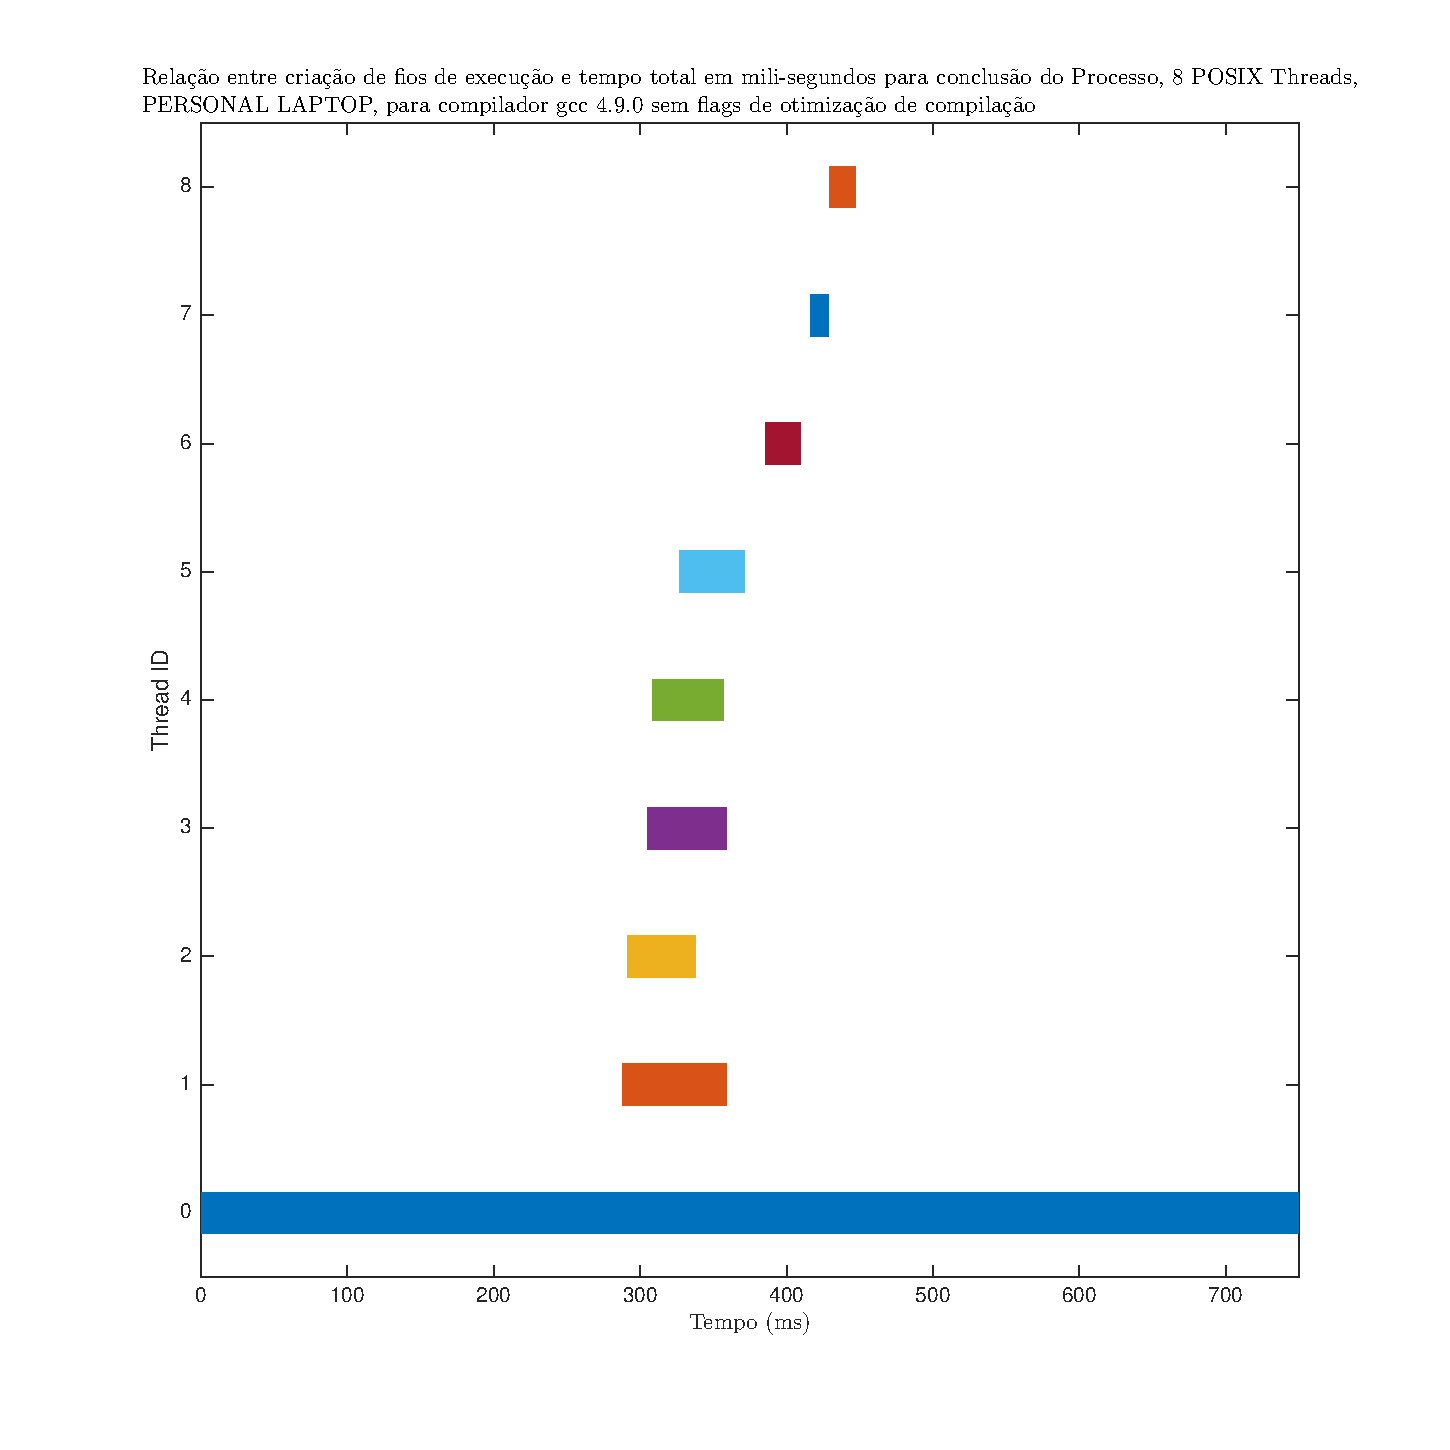
\includegraphics[width=1.1\columnwidth]{EPS/time_create_8T.eps}
\caption{Relação entre criação de fios de execução e tempo total em mili-segundos para conclusão do Processo, 8 POSIX Threads, para o student laptop, para compilador gcc 4.9.0 sem flags de otimização. \textbf{Nota: Thread 0 refere-se ao processo.}}
\label{fig:create_8}
\end{figure}


\begin{figure}[H]
\centering
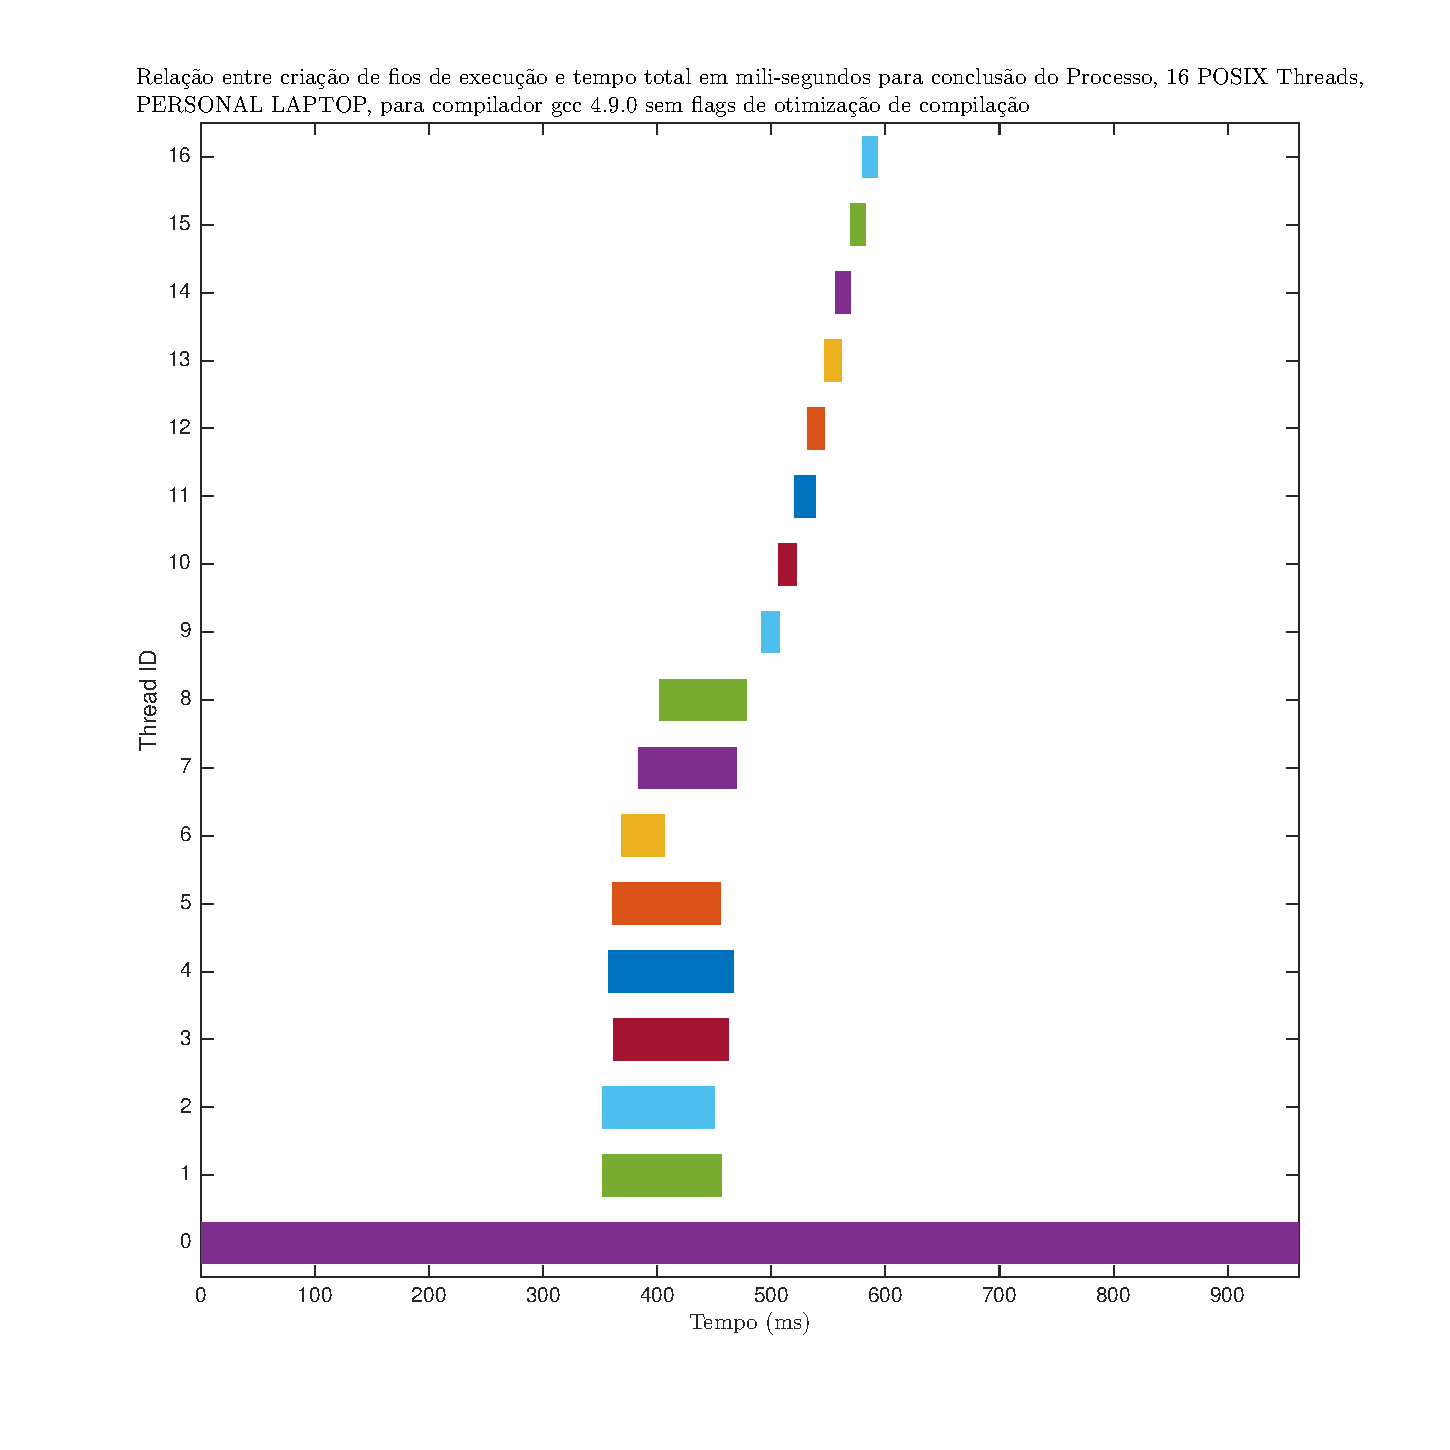
\includegraphics[width=1.1\columnwidth]{EPS/time_create_16T.eps}
\caption{Relação entre criação de fios de execução e tempo total em mili-segundos para conclusão do Processo, 16 POSIX Threads, para o student laptop, para compilador gcc 4.9.0 sem flags de otimização. \textbf{Nota: Thread 0 refere-se ao processo.}}
\label{fig:create_16}
\end{figure}

\begin{figure}[H]
\centering
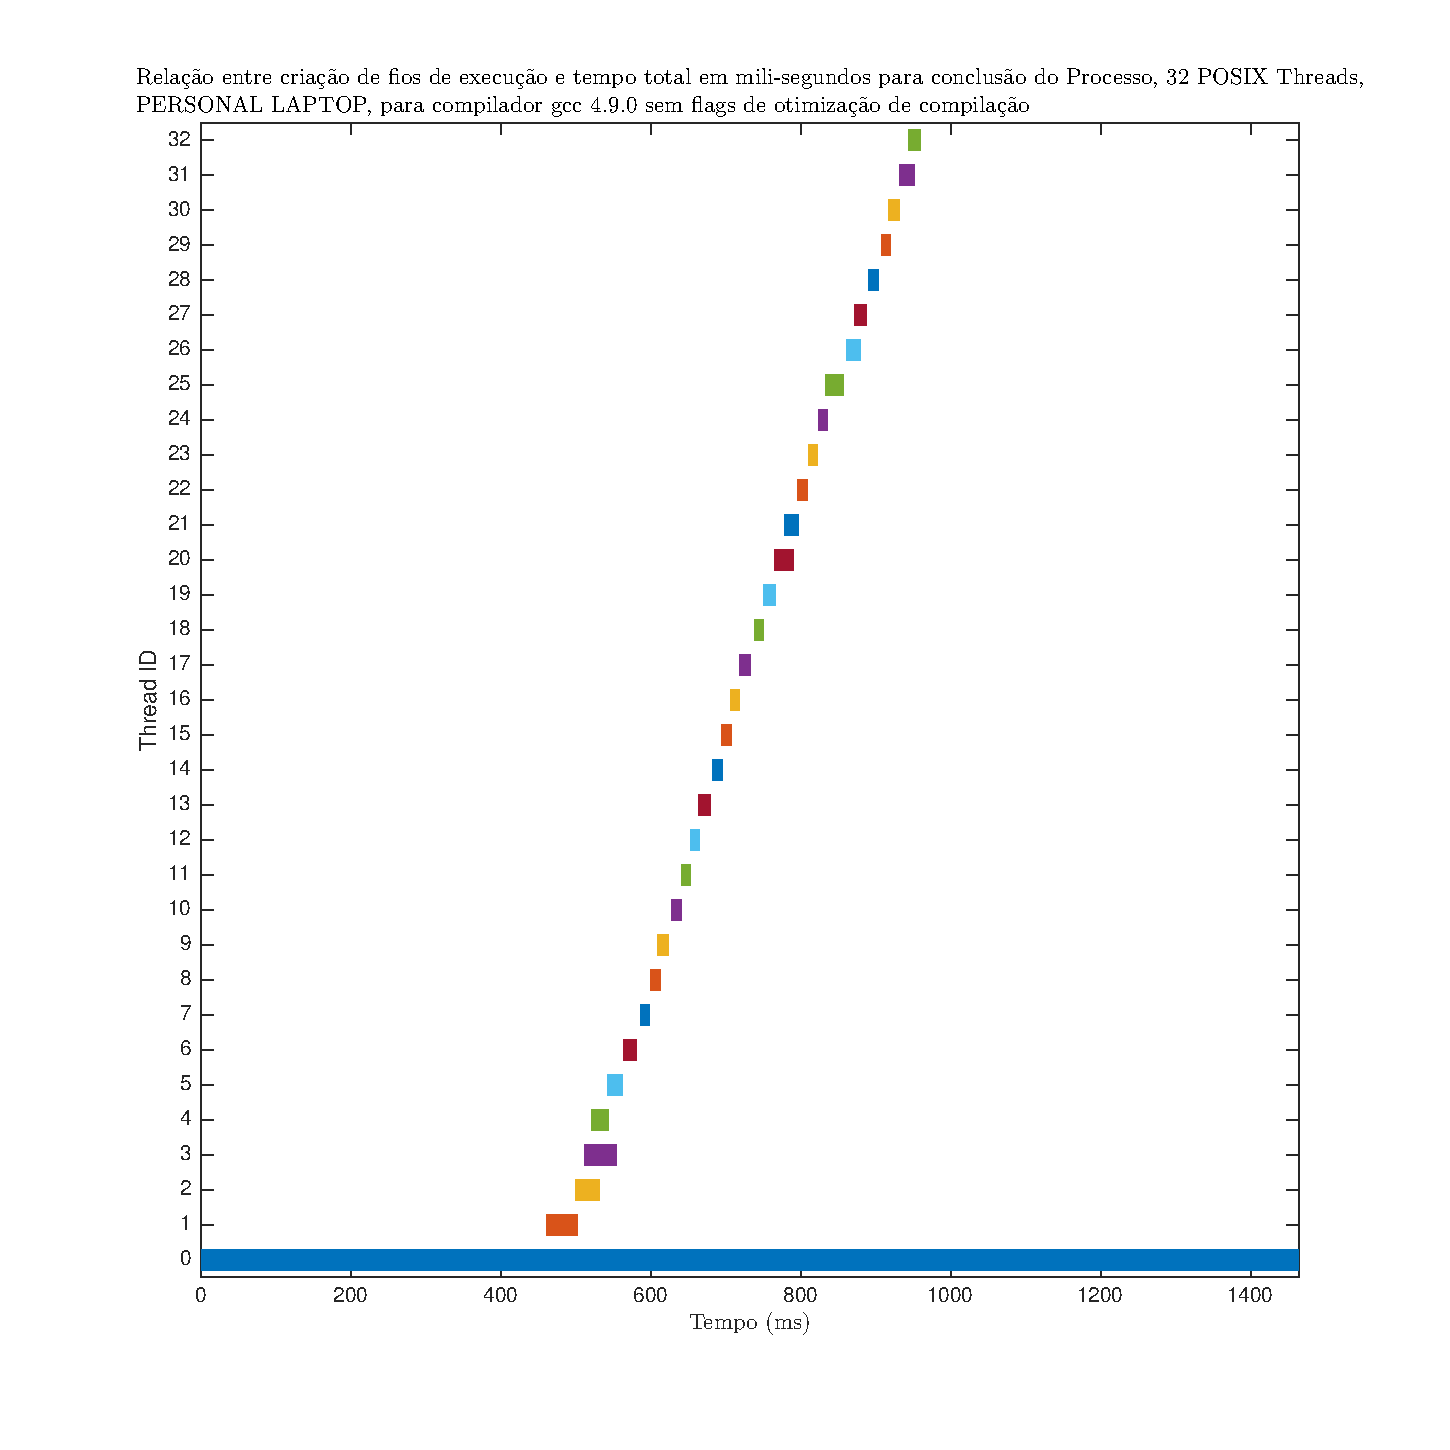
\includegraphics[width=1.1\columnwidth]{EPS/time_create_32T.eps}
\caption{Relação entre criação de fios de execução e tempo total em mili-segundos para conclusão do Processo, 32 POSIX Threads, para o student laptop, para compilador gcc 4.9.0 sem flags de otimização. \textbf{Nota: Thread 0 refere-se ao processo. }}
\label{fig:create_32}
\end{figure}

Denote que para todos os casos distintos, é na inicialização/terminação das primeiras POSIX Threads que despendemos a maior porção de tempo associado às threads -- tal como pode ser confirmado na tabela \ref{table:student_create}. Podemos ainda inferir que o pior resultado registado em termos de tempo total para a solução se dá para o número de POSIX Threads igual a 16 ( o dobro do número de threads físicas disponíveis no CPU ), e que é para um número de POSIX Threads igual a 128 que obtemos tanto o menor desvio como o melhor valor em termos de média. Para a média esta afirmação é válida tanto para os nós compute-431 como para o student laptop. \par 

\begin{table}[H]
\caption{Relação entre média e desvio padrão de criação/terminação para um diferente número de posix threads para o student laptop}
     \label{table:student_create}
\centering
  \begin{tabular}{ | l | r |  r |   }
  
    \hline
    \# POSIX Threads & Média de Criação/Term.  (em $\mu$s) & Desvio P. \\ \hline 
    
1& 23.3620 & 0 \\
2 &  24.7585 & 2.3342 \\
4 & 40.1410 &    10.7082 \\
8 &    39.8469 & 19.8955 \\
16 &    51.6829 &    41.1291 \\
32 &    17.6375  &  7.8276 \\
64 &     26.5381   & 11.5596 \\ 
128 &     14.6927  &     7.8023 \\
256 &     16.7902 &      9.2130 \\
\hline 
  \end{tabular}
\end{table}

Podemos portanto concluir que um aumento no número de fios criados/terminados por um processo leva a uma diminuição do tempo médio necessário para a realização de tais operações, contribuindo ainda para um estabilização desse mesmo tempo em intervalos com uma desvio padrão menor.
%Resta-nos analisar graficamente o comportamento enumerado na tabela \ref{table:student_create}.


\section{Implementação da regra trapezoidal }
Tal como referimos anteriormente, nesta fase iremos submeter a controlo de métricas de performance  3 kernels paralelos, cada um implementando o mesmo algoritmo - \textbf{regra trapezoidal} - com a ressalva para a forma de exclusão mútua de uma secção crítica do mesmo. Iremos recorrer portanto ao método de espera-activa (busy-wait), MUTEX, e Semáforos, e registar a influência de cada escolha no tempo total para o tempo da solução. \par 
Ora, no nosso algoritmo existe apenas uma seção crítica, sendo esta a adição de uma valor calculado a cada iteração das POSIX Threads envolvidas na solução a uma variável global a todas as Threads. \par
Foi escolhido a não recorrência a flags de otimizição uma vez que, para o kernel que implementa a exclusão mútua via espera-activa, otimizações automáticas como a execução fora de ordem de instruções podem levar a situações de dead-lock. Ora, assim e dado que necessitamos de comparar todos os kernels com iguais flags de compilação nenhum dos 3 kernels apresenta otimizações.\par 
Atente no gráfico \ref{fig:time_all}. Como se pode confirmar, a melhor solução para um elevado número de POSIX Threads é alcançada recorrendo a MUTEX's. Ora, podemos considerar que os MUTEX's como um tipo especial de semáforos (semáforos binários), sendo portanto esperado que os valores alcançados pelo método que implementa exclusão mútua via semáforos apresentasse a mesma ordem de grandeza de valores dos apresentados pelo kernel que implementa a exclusão mútua via MUTEX's. Contudo, tal não se verifica, tendo o kernel  implementado recorrendo a semáforos os mesmos fracos resultados que os apresentados pelo kernel que implementa espera-activa.\par 
Ora, esta grande diferença poderá estar relacionada como o facto de num MUTEX's apenas a Thread que bloqueou a variável de condição a pode desbloquear. Talvez por essa premissa se consigam reduções no tempo de verificação da variável de condição e consequentemente melhores resultados.\par 
Não obstante o anteriormente dito resta-nos ressalvar que este algoritmo é demasiado simplista e de fácil resolução da dependência de dados para podermos extrapolar conclusões para qualquer outro algoritmo. No que toca à resolução da necessidade a cada iteração da secção crítica, cada POSIX Thread poderia ter a variável approx local -- \textbf{approx\_local}, sendo apenas esse valor reduzido no final do trabalho de cada thread -- retirando a necessidade de \textbf{n} (no nosso caso 1048576)  operações atómicas, passando apenas a ser necessárias \textbf{n\_threads} (no nosso caso máximo 256) operações atómicas, retirando quase por completo todo o overhead gerado pela operação de adição de valores à variável global (Podemos pensar nesta alteração como a implementação de um conceito map/reduce).


\begin{figure}[H]
\centering
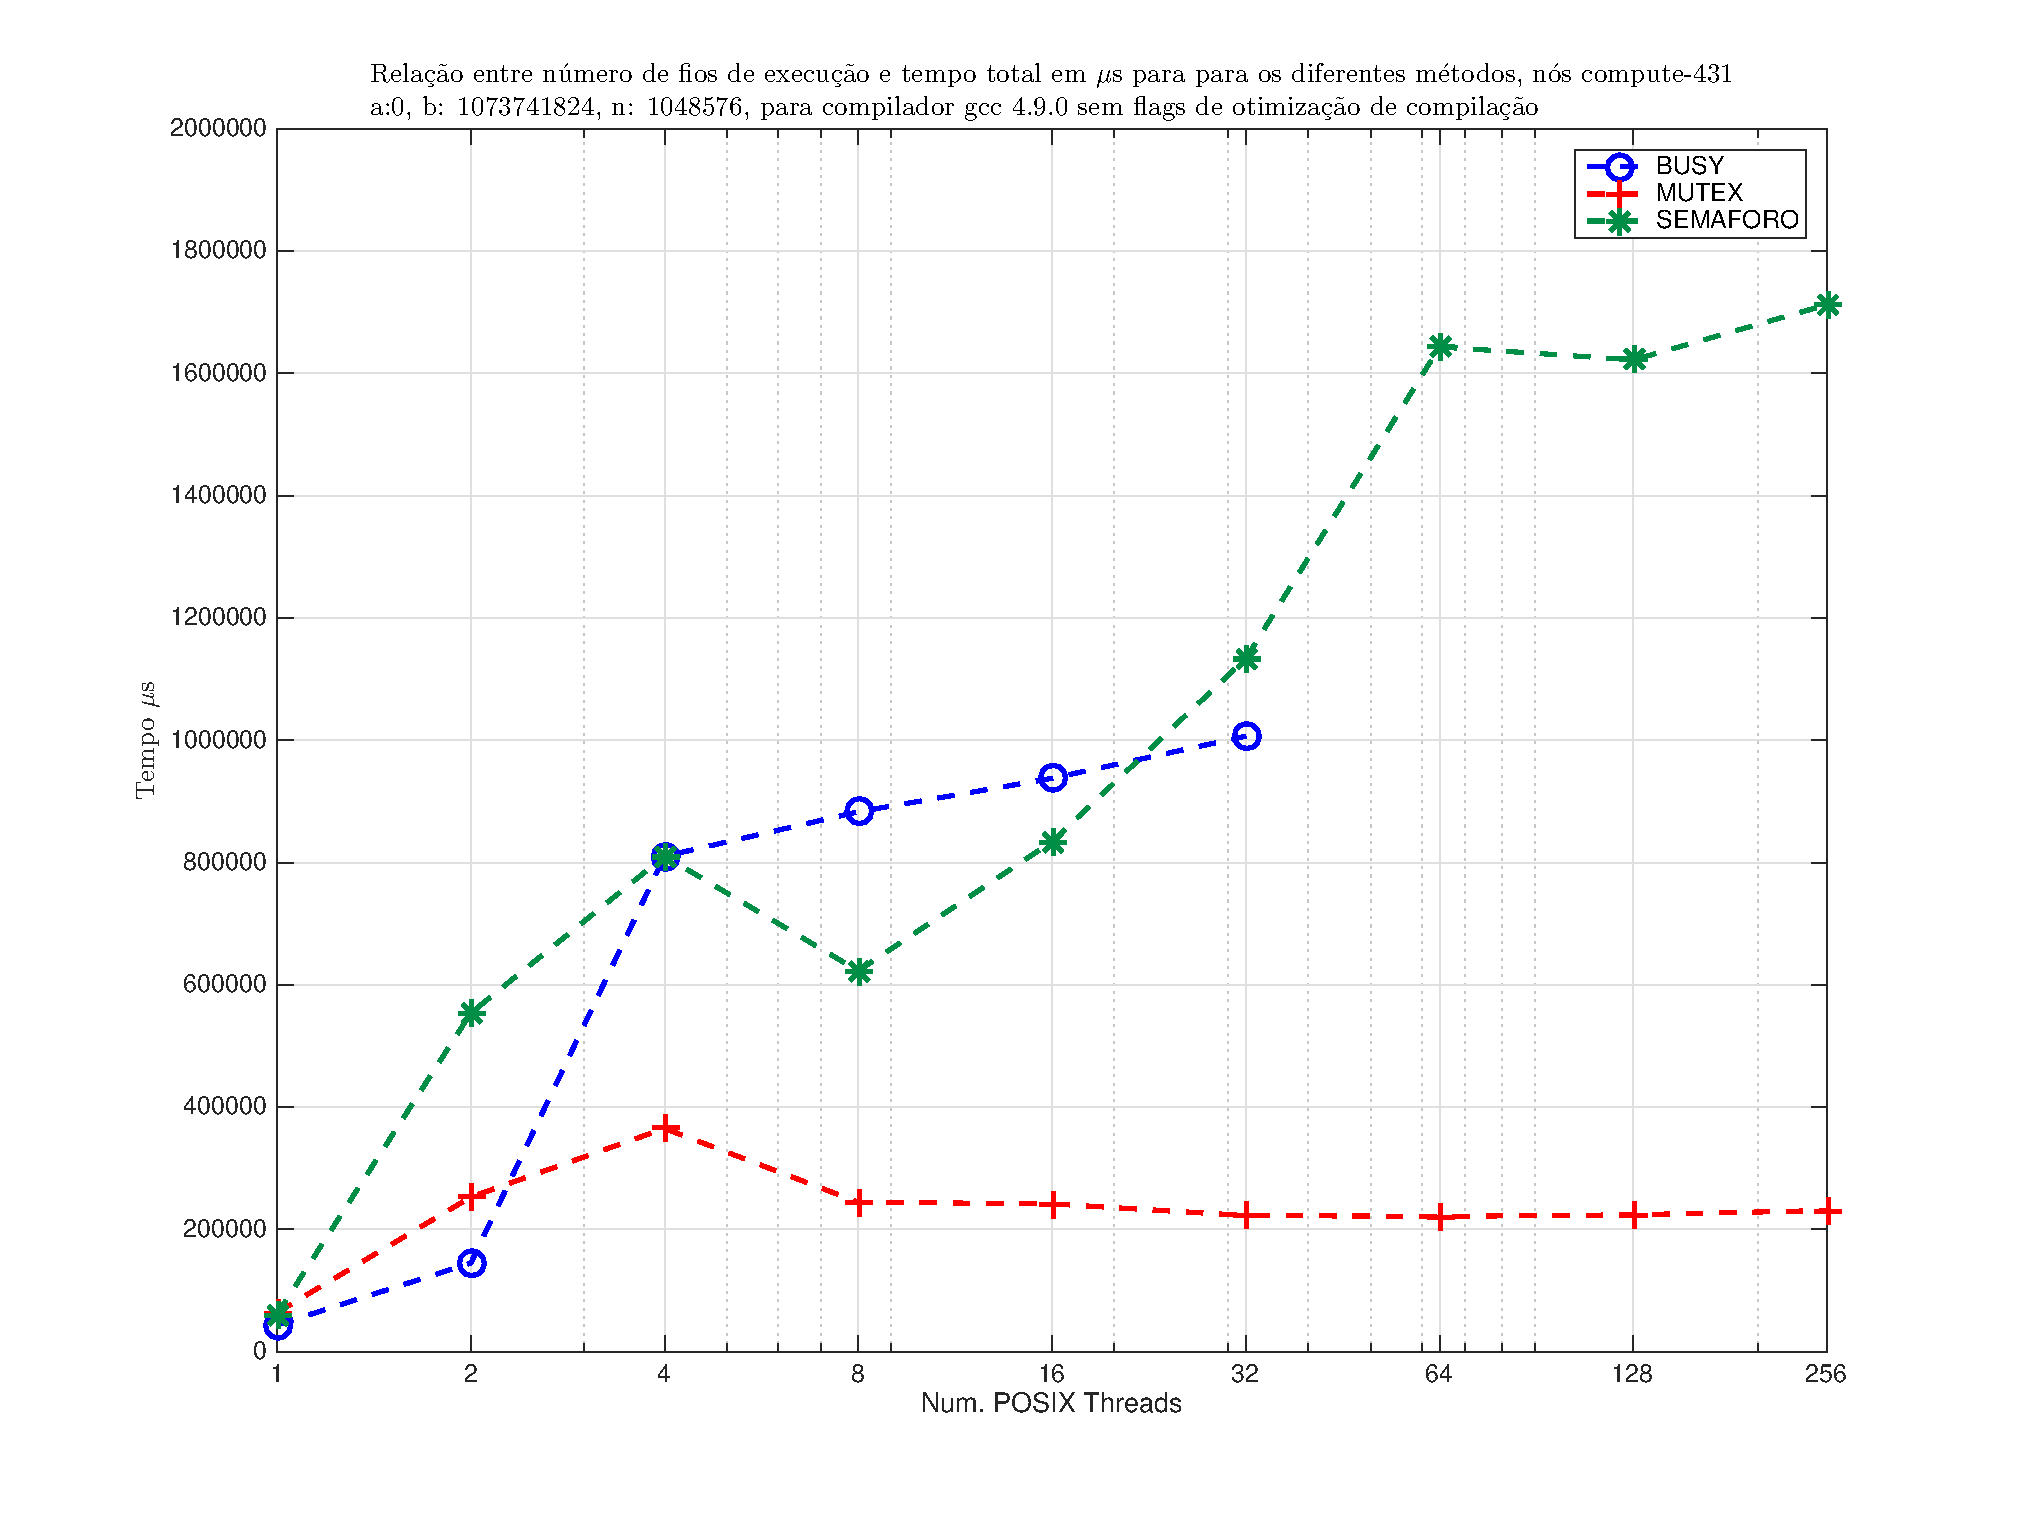
\includegraphics[width=1.1\columnwidth]{EPS/time_all.eps}
\caption{Relação entre criação de fios de execução e tempo total em $\mu$ segundos para conclusão do Processo, para diferentes números de POSIX Threads, para os diferentes métodos de exclusão mútua de secção crítica, para os nós compute-431, para compilador gcc 4.9.0 sem flags de otimização, para a=0, b=1073741824, e n=1048576.  \\{Nota: Para um número de POSIX Threads superior a 32 não foi possível recolher os valores de tempo total em mili-segundos para conclusão do Processo nos nós 431} }
\label{fig:time_all}
\end{figure}

\subsection{Implementação da regra trapezoidal recorrendo a OpenMP (PThreads vs OpenMP)}
Tal como nas POSIX Threads, o OpenMP recorre a uma API para implementação de kernels paralelos em memória partilhada. A grande diferença assenta no "esforço" necessário para paralelizar kernels. Enquanto que via OpenMP através de um conjunto de directivas conseguimos obter código paralelo, recorrendo a PThreads necessitamos de explicitamente especificar o processo de criação, terminação, e comportamento de cada Thread. \par 
Analisemos portanto a facilidade de paralelizar (sem otimizações quer via mudança do algoritmo quer via adição de flags de compilação) o nosso algoritmo:

{\small
\begin{lstlisting}
#pragma omp parallel num_threads(thread_count)
{
  #pragma omp parallel for schedule(static,my_n)
    for (i = interval_a ;i<=interval_b-1;i+=h){
      x_i = interval_a + i*h;
      #pragma omp atomic      
      approx  +=  f(x_i);
    }
}
\end{lstlisting}
}



Por forma a obtermos o mesmo "comportamento" adicionamos o scheduling static e de tamanho my\_n (o mesmo que para o nosso algoritmo implementado via PThreads).


\begin{figure}[H]
\centering
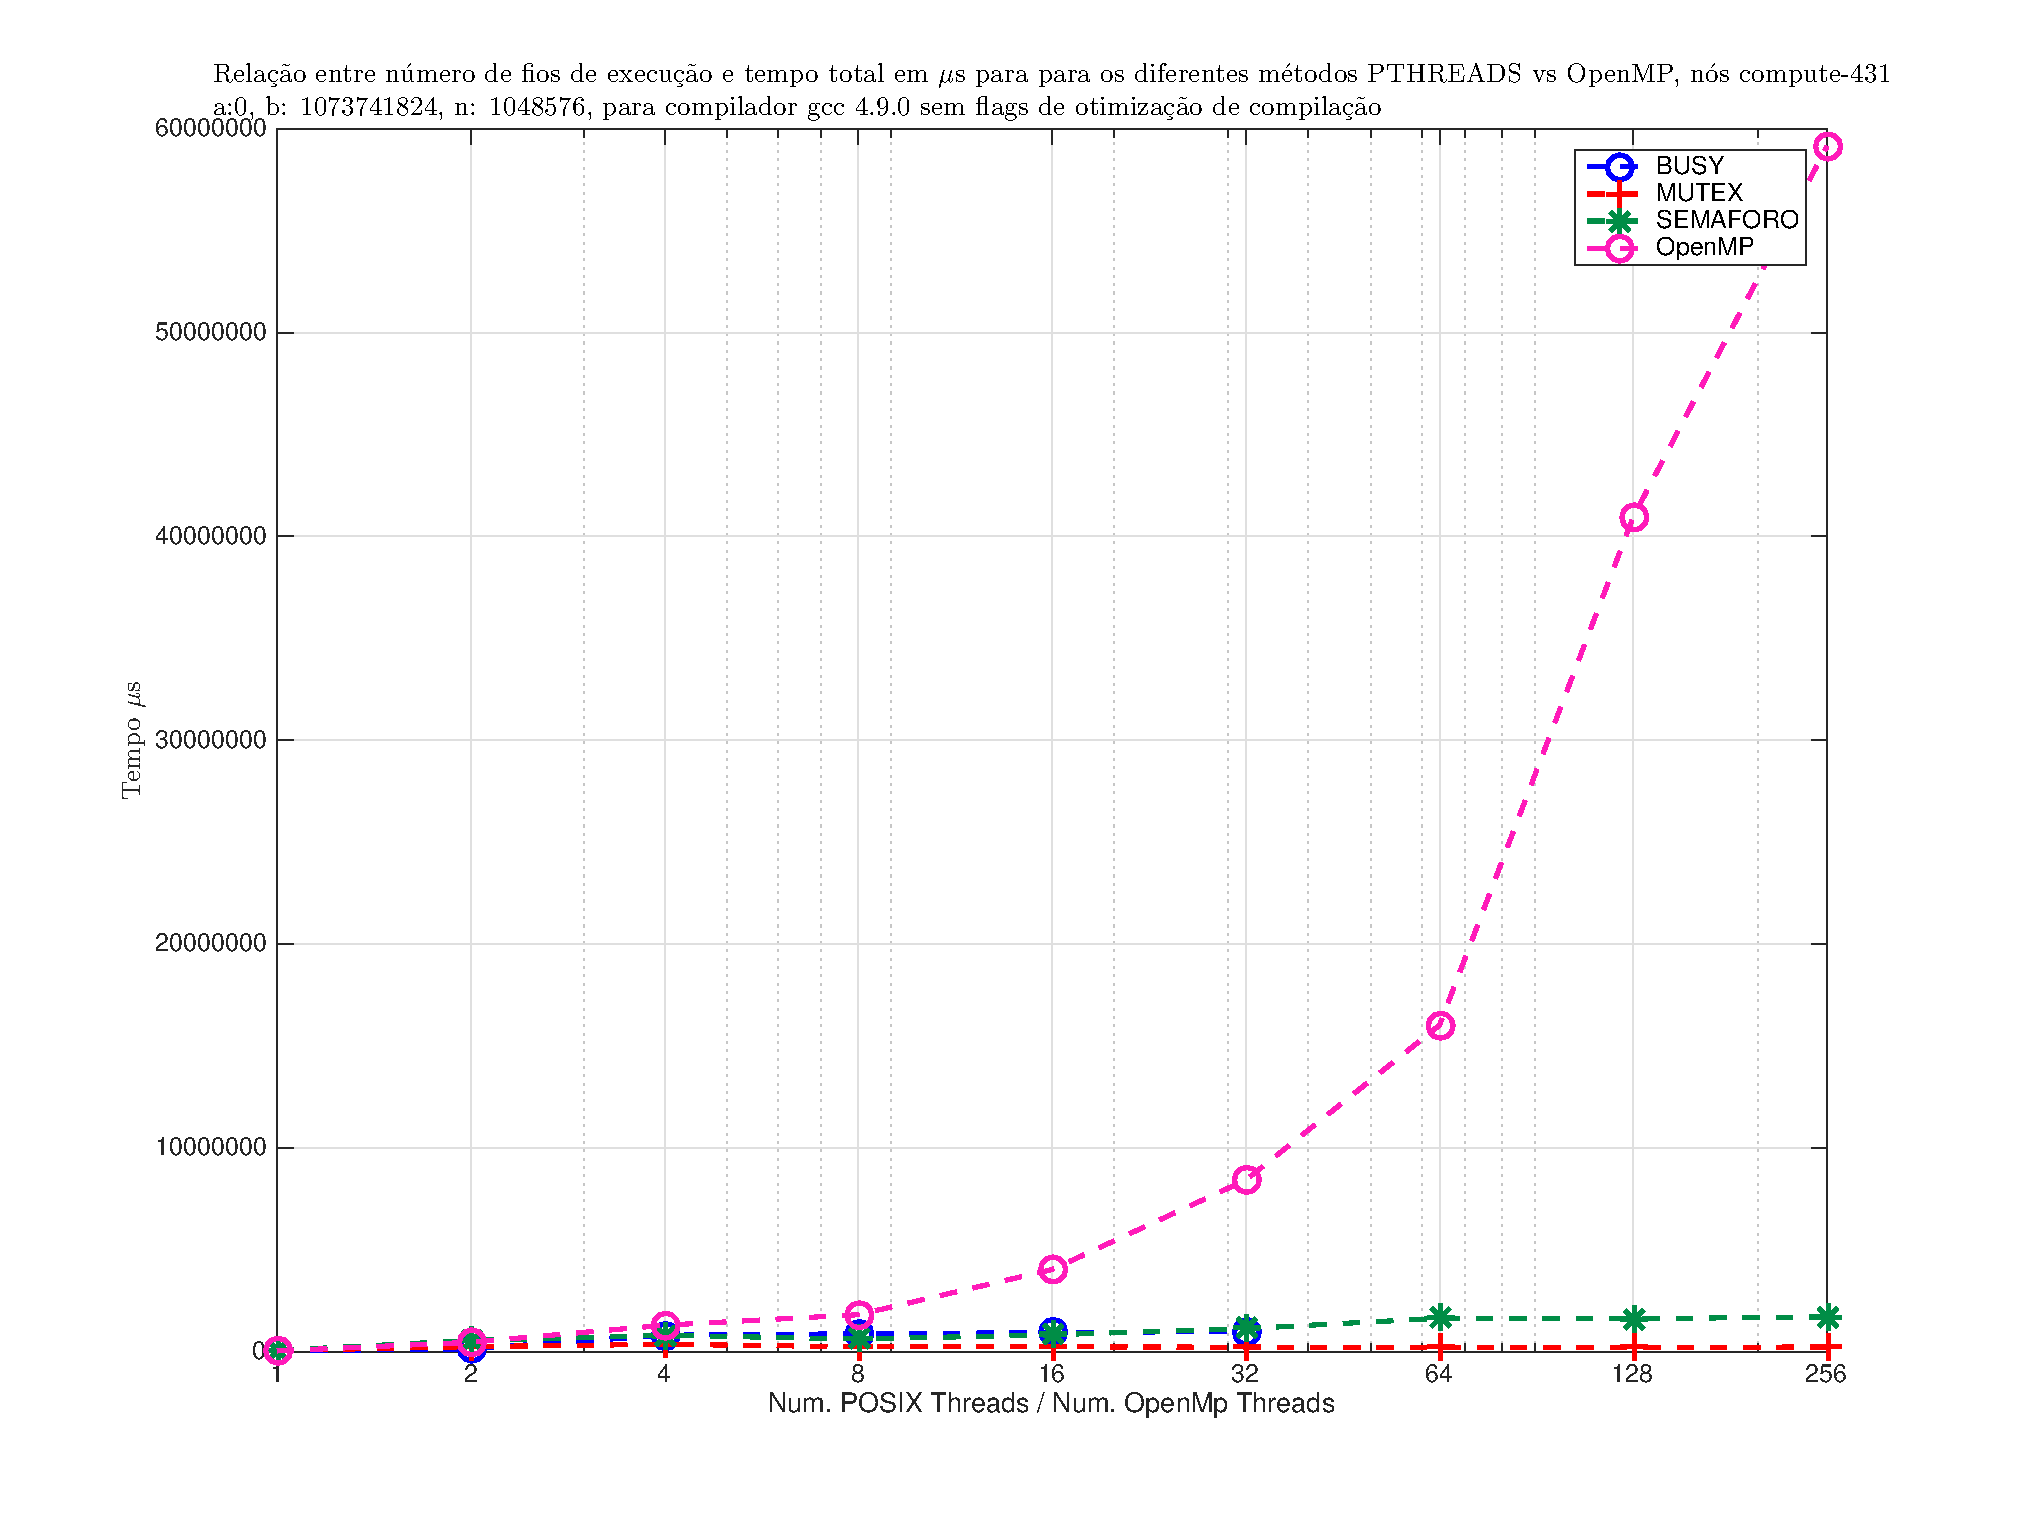
\includegraphics[width=1.1\columnwidth]{EPS/time_omp.eps}
\caption{Relação entre criação de fios de execução e tempo total em $\mu$ segundos para conclusão do Processo, para diferentes números de POSIX Threads / OpenMp Threads, para os diferentes métodos de exclusão mútua de secção crítica, para os nós compute-431, para compilador gcc 4.9.0 sem flags de otimização, para a=0, b=1073741824, e n=1048576.  \\{Nota: Para um número de POSIX Threads superior a 32 não foi possível recolher os valores de tempo total em mili-segundos para conclusão do Processo nos nós 431} }
\label{fig:time_omp}
\end{figure}

As Pthreads são portanto mais "baixo nível" e permitem otimizações e especificação de comportamentos específicos por thread.
Em OpenMP somos confrontados com a "facilidade" de paralelização a custo de por vezes performance (ver figura \ref{fig:time_omp}) e interações de mais baixo nível entre Threads difíceis de computar. \par 
Contudo, não podemos afirmar que o recurso a PThreads é sempre vantajoso -- se necessitarmos de uma otimização máxima e parelelização superior à conseguida através de ciclos e directivas, então deverão ser escolhidas PThreads. Caso seja "suficiente" o grau de paralelismo alcançado com as diretivas OpenMP, dado o pouco esforço necessário à produção de código paralelo simples, então a opção deverá ser a de recorrência a OpenMP. Denote que a paralelização via OpenMP tem ainda a vantagem da  manutenção de código sequencial, bastando para isso compilar sem a flag -fopenmp.

\section{Conclusão}
Relativamente aos kernels em estudo podemos concluir que o recurso a MUTEX's, \textbf{para o nosso caso específico}, se revelou mais vantajoso, mas, tal como referido anteriormente dada a simplicidade do algoritmo não se podem retirar conclusões acerca da generalidade de mecanismos de exclusão mútua.
Neste caso também se verificou um ganho de performance relativamente à paralelização em ambiente de memória partilhada via OpenMP, por si só espectável -- o overhead de criação das zonas paralelas, dado o pouco de recurso do algoritmo a ciclos (apenas 1) não se verificou compensatório.\par 
O valor do algoritmo deste caso de estudo ultrapassa os resultados obtidos, prendendo-se uma vez mais com o desenvolvimento e prática de ferramentas (\textbf{dtrace}), e métodos de tratamento e análise de métricas de sistemas de computação de alta perfomance, assim como uma forma de maior ambientação no ambiente de clustering presente no Search6.









% conference papers do not normally have an appendix



% use section* for acknowledgment
%\ifCLASSOPTIONcompsoc
  % The Computer Society usually uses the plural form
 % \section*{Acknowledgments}
%\else
  % regular IEEE prefers the singular form
  %\section*{Acknowledgment}
%\fi


%The authors would like to thank...





% trigger a \newpage just before the given reference
% number - used to balance the columns on the last page
% adjust value as needed - may need to be readjusted if
% the document is modified later
%\IEEEtriggeratref{8}
% The "triggered" command can be changed if desired:
%\IEEEtriggercmd{\enlargethispage{-5in}}

% references section

% can use a bibliography generated by BibTeX as a .bbl file
% BibTeX documentation can be easily obtained at:
% http://mirror.ctan.org/biblio/bibtex/contrib/doc/
% The IEEEtran BibTeX style support page is at:
% http://www.michaelshell.org/tex/ieeetran/bibtex/
%\bibliographystyle{IEEEtran}
% argument is your BibTeX string definitions and bibliography database(s)
%\bibliography{IEEEabrv,../bib/paper}
%
% <OR> manually copy in the resultant .bbl file
% set second argument of \begin to the number of references
% (used to reserve space for the reference number labels box)


%\begin{thebibliography}{1}

%\%bibitem{nas}
%NAS Parallel Benchmarks, \url{http://www.nas.nasa.gov/publications/npb.html}

%\end{thebibliography}

%\appendix 


% that's all folks
\end{document}


